\begin{frame}[plain]
  \centering
  \vspace*{0.18\paperheight}
  \LARGE \textbf{Fine-Tuning Methods for LLMs}
\end{frame}

\begin{frame}{Categories of Fine-Tuning}
  \begin{center}
    \small
    \renewcommand{\arraystretch}{1.4}
    \begin{tabular}{|l|>{\raggedright\arraybackslash}p{5.6cm}|c|c|}
      \hline
      \textbf{Method} & \textbf{Description} & \textbf{Trained params} & \textbf{Cost} \\
      \hline
      Full FT & Retrain all weights & All & Expensive \\
      Adapter & Insert small bottleneck layers (Houlsby et al., 2019) & Few & Efficient \\
      Prefix / Prompt & Tune continuous prompt vectors, base model frozen & Few tokens & Efficient \\
      LoRA / QLoRA & Low-rank weight deltas & Very few & Very efficient \\
      Instruction tuning & Tune on instruction-response datasets & All or part & Varies \\
      \hline
    \end{tabular}
  \end{center}
  \vspace{0.4em}
  {\scriptsize Instruction tuning is an orthogonal axis: it describes \emph{what data} the model is tuned on, and can be done with any of the methods above.}
\end{frame}

\begin{frame}[t]{Full Fine-Tuning (FT)}
  \begin{itemize}
    \item[\textcolor{red}{$\blacktriangleright$}] \textbf{Definition:} Fine-tune all parameters of the pre-trained model on downstream data.
    \item[\textcolor{red}{$\blacktriangleright$}] \textbf{Historical Use:} Common in early GPT-2 and BERT applications.
    \item[\textcolor{red}{$\blacktriangleright$}] \textbf{Pros:}
      \begin{itemize}
        \item Maximum flexibility and performance
      \end{itemize}
    \item[\textcolor{red}{$\blacktriangleright$}] \textbf{Cons:}
      \begin{itemize}
        \item Expensive (requires large compute resources)
        \item Prone to catastrophic forgetting
        \item Not efficient for large models
      \end{itemize}
  \end{itemize}
\end{frame}

\begin{frame}{Full Fine-Tuning Workflow}
  \begin{figure}
    \centering
    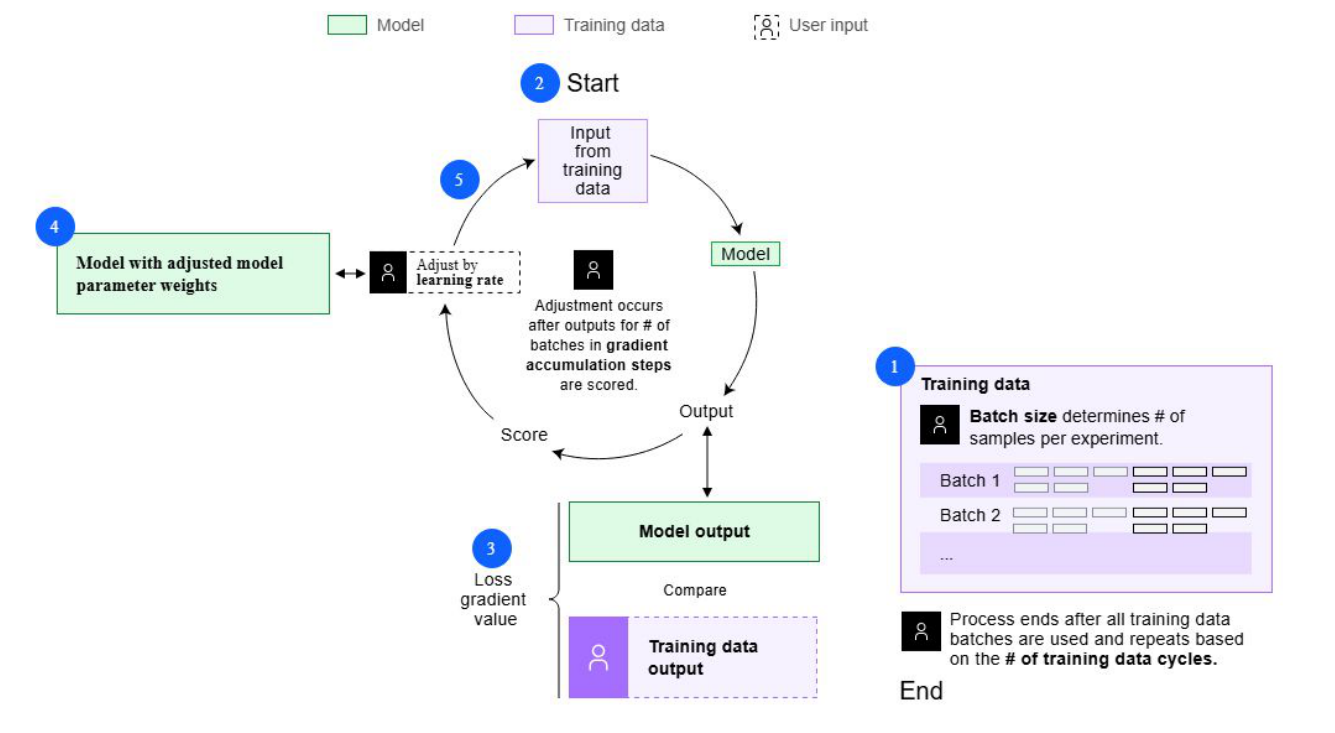
\includegraphics[width=0.74\paperwidth,height=0.60\paperheight,keepaspectratio]{images/llm-rlhf/finetune_training_loop_batches.png}
    \caption*{\scriptsize Source: IBM watsonx.ai documentation, ``Full fine tuning,'' \url{https://www.ibm.com/docs/en/watsonx/w-and-w/2.1.0?topic=tuning-full-fine}.}
  \end{figure}
\end{frame}

\begin{frame}{Parameter-Efficient Fine-Tuning (PEFT)}
  \begin{itemize}
    \item[\textcolor{red}{$\blacktriangleright$}] \textbf{Key Idea:} Keep the base model frozen, tune only a small subset of parameters.
    \item[\textcolor{red}{$\blacktriangleright$}] \textbf{Types:}
    \begin{itemize}
      \item Adapter Modules (Houlsby et al., 2019)
      \item Prefix Tuning (Li \& Liang, 2021) and Prompt Tuning (Lester et al., 2021)
      \item LoRA / QLoRA
    \end{itemize}
    \item[\textcolor{red}{$\blacktriangleright$}] \textbf{Benefits:}
    \begin{itemize}
      \item Enables multi-tasking and personalization
      \item Suitable for low-resource adaptation
      \item Reduces compute and memory requirements
    \end{itemize}
  \end{itemize}
\end{frame}


\begin{frame}{Parameter-Efficient Fine-Tuning (PEFT)}
  \centering
  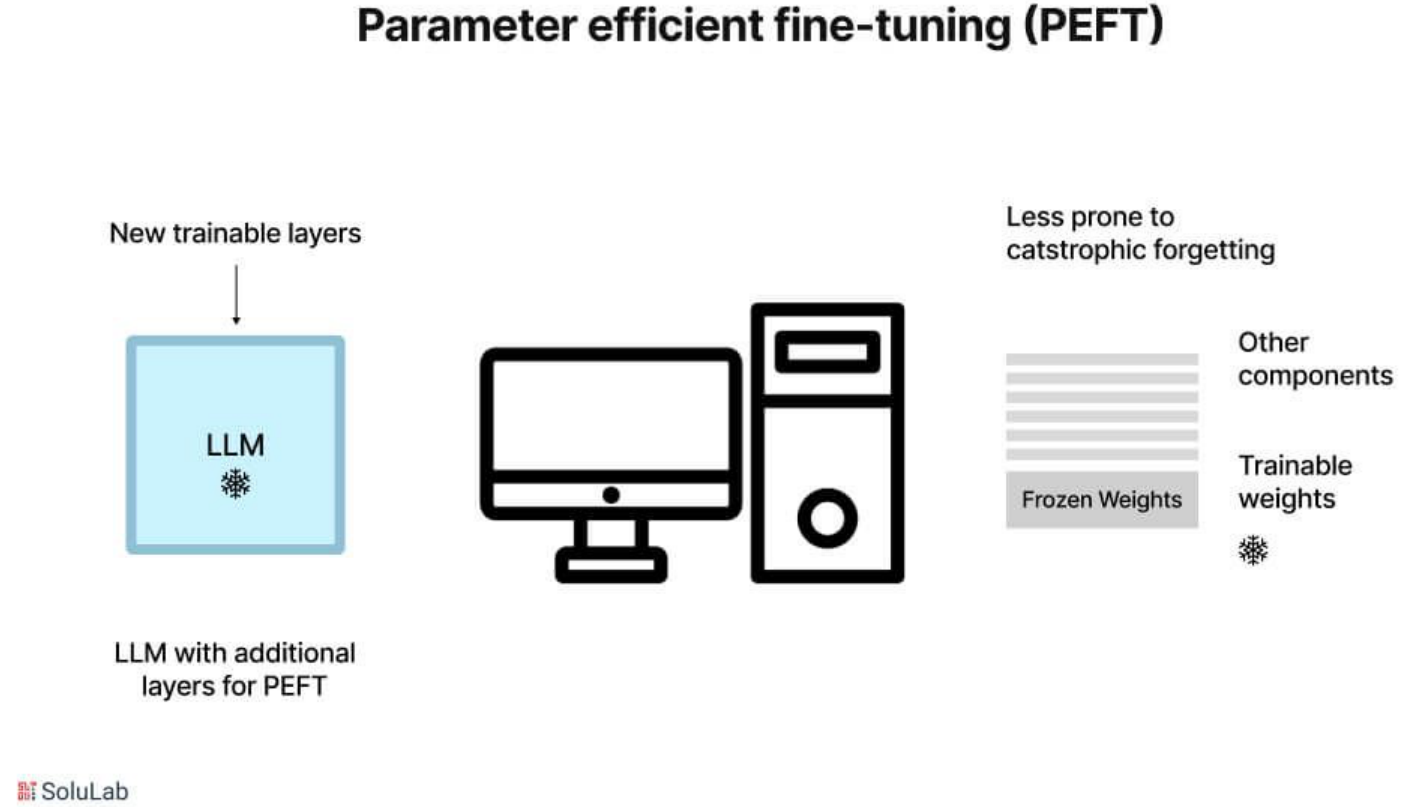
\includegraphics[width=0.60\paperwidth,height=0.60\paperheight,keepaspectratio]{images/llm-rlhf/finetune_peft_overview.png}
\end{frame}
